\documentclass[a4paper,twoside]{article}
\usepackage[utf8]{inputenc}
\usepackage{url}
\usepackage{color}
\usepackage{charter}
\usepackage{caption}
\usepackage{parskip}
\usepackage{graphicx}
\usepackage[margin=1in]{geometry}
%
%
\newcommand{\shortstandard}{ISO/IEC~18004}
\newcommand{\standard}{\shortstandard:2024(en)}
\newcommand{\quotestandard}[1]{\textcolor{blue}{\textit{#1}}}
\newcommand{\ddd}{\dots}
\newcommand{\change}[1]{\underline{\textbf{#1}}}
\newcommand{\hex}[1]{#1(hex)}

\newcommand{\best}[1]{\underline{#1}}
\newcommand{\good}[1]{\textcolor{green}{#1}}
\newcommand{\bad}[1]{\textcolor{red}{#1}}
%
%
\captionsetup{margin=10pt,font={small,it}} % Options: tiny, scriptsize, footnotesize, small, normalsize, etc.
%
%
\title{Suggested improvements to \standard}
\author{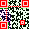
\includegraphics[width=0.2\textwidth]{images/email.png} \\ \\ Sidney~Cadot~\url{<sidney.cadot@gmail.com>}\footnote{The author wishes to acknowledge Joris~van~Rantwijk for the many fruitful discussions about the
precise meaning of some sections in the QR code standard, and for proofreading this document. Joris wrote a QR code \emph{decoder} a few years ago, so his insights nicely complemented my own experience on the encoder side.}}
\date{Version 1.0.1 --- May~31\textsuperscript{st},~2025}
%
%
\begin{document}
%
\maketitle
\tableofcontents
%
\section{Introduction}

The \standard{} standard describes the encoding and decoding of QR code symbols. With this standard in hand,
I recently implemented a QR code encoder library\footnote{The encoder I implemented can be found on Github:
\url{https://github.com/sidneycadot/qrcodes}.}, mostly to satisfy my curiosity about how QR codes work.

To implement a working encoder, a close reading of the standard was necessary. With the benefit of reading
with a `fresh pair of eyes', several suspected mistakes were found:

\begin{itemize}
\item The Data Mask Pattern selection procedure appears to be incorrectly applied in four of the seven
      QR code symbols shown in the standard.
      This issue is described in Section~\ref{sec:data-mask-pattern-selection}.
\item The procedure for dealing with mirrored QR codes as described in the standard leads to a failure
      to correctly decode mirrored QR codes in most cases.
      This issue is described in Section~\ref{sec:mirrored-symbol-issue}.
\item A number of trivial syntactic mistakes were found.
      These are listed in Section~\ref{sec:trivial-issues}.
\end{itemize}

Apart from these issues, there are several other places where it may be possible to improve the clarity
of the standard. In the interest of brevity these are not currently included in this document. If useful,
I can present a list of these at a later stage.

%My hope is that the standard committee will consider the issues described in this document, and that at
%least some of those will lead to improvements in the next edition of the standard.

\section{Data Mask Pattern selection and the standard's QR code symbols}
\label{sec:data-mask-pattern-selection}

Section~7.8.3.1 of \standard\ describes a scoring procedure for QR code symbols using eight different
Data Mask Patterns, with the goal of selecting the pattern that is least likely to confuse QR code readers.

\subsection{Wording of the scoring procedure}

Section~7.8.3.1 is quite terse and several parts of it are hard to understand.

The sentence fragment below from the introductory paragraph is somewhat confusing:

\begin{quote}
\quotestandard{\ddd the variables N1 to N4 represent weighted penalty scores for the undesirable features \ddd}
\end{quote}

However, N1 to N4 are not variables, but \emph{constants}; and they don't represent weighted penalty
scores, as claimed; rather, they are merely constants used in the calculation of the four terms that make
up the final penalty score for a given symbol.

Another issue is that there is an ambiguity in this section with regard to the calculation of the first score term.
In NOTE~1 it is first said that blocks consisting of \emph{more than five} modules are checked, but later on
it is stated that a five-module block counts for three points.

The clarity of this section could be greatly improved if one or two concrete examples were added that show the four
terms contributing to the penalty score, as well as the final scores, for each of the eight data mask patterns.

An example of what that could look like is shown in Table~\ref{tab:dmp-selection-annex-example} below.
For the QR code symbol discussed in Annex~I, it shows the exact score contributions and the total score for each
of the eight data patterns.

\begin{table}[h!]
\centering
\small
\begin{tabular}{|c|c|c|c|c|c|}
\hline
Data mask pattern & 1st score term & 2nd score term & 3rd score term & 4th score term & Total score \\
\hline
Pattern 0            & 182              & 171               & 800              &  0                & 1153        \\
Pattern 1            & 216              & 234               & 800              &  0                & 1250        \\
Pattern 2            & 235              & 195               & 720              & 10                & 1160        \\
Pattern 3            & 216              & 192               & 720              &  0                & \best{1128} \\
Pattern 4            & 217              & 237               & 760              &  0                & 1214        \\
Pattern 5            & 245              & 228               & 760              & 10                & 1243        \\
Pattern 6            & 207              & 186               & 760              &  0                & 1153        \\
Pattern 7            & 203              & 210               & 720              &  0                & 1133        \\
\hline
\end{tabular}
\caption{Partial and total scores for the QR code discussed in Annex~I}
\label{tab:dmp-selection-annex-example}
\end{table}

\subsection{Some Data Mask Patterns in the standard's QR code examples are incorrect}

The standard contains seven QR code symbol examples: one in Figure~1, five in Figure~29, and one in Figure~I.2.

Unfortunately, the Data Mask Pattern used in those symbols does not always correspond to the Data Mask Pattern
with the lowest score, which is confusing for implementers that try to reproduce those examples to validate
their own implementation.

Table~\ref{tab:dmp-selections} shows the scores calculated according to the scoring method described in Section~7.8.3.1,
for each of the seven QR codes found in the standard, and for each of the eight data mask pattern choices.
Also listed is the optimal data mask pattern choice (with the  lowest score) and the data mask pattern actually
used in the QR code symbol shown in the standard.

These two data mask pattern choices should match, but for four out of seven cases, they do not.

\begin{table}[h!]
\centering
\tiny
\begin{tabular}{|c|c|c|c|c|c|}
\hline
QR code example & Description & Symbol & Pattern scores P0 to P7 (best score underlined) & Optimal pattern & Pattern used in standard \\
\hline
Figure 1              & ``QR Code Symbol''                       & 1-M & 1219,1195,1189,1182,1142,\best{1107},1116,1198 & Pattern 5 & \bad{Pattern 6}  \\
Figure 29, top        & Structured Append Mode example, combined & 4-M & 1672,1684,1568,\best{1402},1416,1690,1598,1624 & Pattern 3 & \bad{Pattern 4}  \\
Figure 29, second row & Structured Append Mode example, 1 of 4   & 1-M & \best{1097},1146,1208,1174,1136,1164,1184,1128 & Pattern 0 & \good{Pattern 0} \\
Figure 29, second row & Structured Append Mode example, 2 of 4   & 1-M & \best{1095},1192,1203,1167,1133,1178,1171,1103 & Pattern 0 & \bad{Pattern 7}  \\
Figure 29, second row & Structured Append Mode example, 3 of 4   & 1-M & 1119,1125,1191,1134,1196,1137,1123,\best{1090} & Pattern 7 & \good{Pattern 7} \\
Figure 29, second row & Structured Append Mode example, 4 of 4   & 1-M & 1245,1173,1207,\best{1128},1148,1155,1172,1136 & Pattern 3 & \good{Pattern 3} \\
Figure I.2            & ``01234567''                             & 1-M & 1153,1250,1160,\best{1128},1214,1243,1153,1133 & Pattern 3 & \bad{Pattern 2} \\
\hline
\end{tabular}
\caption{Overview of the QR code symbols found in \standard\ and their data mask pattern choices}
\label{tab:dmp-selections}
\end{table}

\subsection{Missing tie-breaker rule}

The standard does not currently specify a tie-breaker rule in case two data mask patterns yield an identical score.

Such a rule could be very simple, e.g., `in case of multiple data mask pattern choices having the same score, select
Pattern~0 over Pattern~1, Pattern~1 over Pattern~2, and so on', or something to that effect.

This would ensure that, for each QR code, there is a fully deterministic and unambiguous way of selecting the correct data mask pattern.

\section{The prescribed procedure for handling mirrored QR codes leads to decoding failures}
\label{sec:mirrored-symbol-issue}


The handling of mirrored QR code symbols was introduced in the 2006 edition of the standard. The procedure to determine if a QR code symbol
is mirrored is described in \standard, Clause~11~part~(b), and Clause~12~parts~(j) and (k).

The prescribed procedure to determine if the QR code symbol being decoded is \emph{normal} or \emph{mirrored} can be summarized as follows:

\begin{itemize}
\item Inspect the format information bits. If (after error correction) it is correct, proceed with decoding under the assumption that the symbol
      is \emph{normal} (i.e., non-mirrored).
\item If not, try to reverse the order of the format information bits, and see if (after error correction) that yields an acceptable format information
      codeword. If so, proceed with decoding under the assumption that the symbol is \emph{mirrored}.
\item If not, declare failure. 
\end{itemize}

The problem with this procedure is that the reverse-order bit string of most encoded format information words decode to another valid format information word, with a Hamming
distance equal to 3. Table~\ref{tab:format-information-bit-reversal} on the next page shows for which of the 32 possible format information bit patterns this happens.

Hence, based on the format information alone, and allowing for 3 incorrect (inverted) modules, it is not possible to make a reliable determination of
whether the QR code symbol being decoded is mirrored or not.

\begin{table}[h!]
\centering
\begin{tabular}{|c|c|c|c|c|}
\hline
entry & data bits & sequence after masking & sequence after matching, reversed & unintended match \\
\hline
 0 & 00000 & 101010000010010 & 010010000010101 & \bad{entry 28} \\
 1 & 00001 & 101000100100101 & 101001001000101 & \bad{entry 21} \\
 2 & 00010 & 101111001111100 & 001111100111101 & \bad{entry 26} \\
 3 & 00011 & 101101101001011 & 110100101101101 & \bad{entry 31} \\
 4 & 00100 & 100010111111001 & 100111111010001 & \bad{entry 6} \\
 5 & 00101 & 100000011001110 & 011100110000001 & \bad{entry 29} \\
 6 & 00110 & 100111110010111 & 111010011111001 & \bad{entry 4} \\
 7 & 00111 & 100101010100000 & 000001010101001 & \bad{entry 16} \\
 8 & 01000 & 111011111000100 & 001000111110111 & \textit{n/a} \\
 9 & 01001 & 111001011110011 & 110011110100111 & \bad{entry 12} \\
10 & 01010 & 111110110101010 & 010101011011111 & \bad{entry 30} \\
11 & 01011 & 111100010011101 & 101110010001111 & \textit{n/a} \\
12 & 01100 & 110011000101111 & 111101000110011 & \bad{entry 9} \\
13 & 01101 & 110001100011000 & 000110001100011 & \bad{entry 18} \\
14 & 01110 & 110110001000001 & 100000100011011 & \textit{n/a} \\
15 & 01111 & 110100101110110 & 011011101001011 & \bad{entry 24} \\
16 & 10000 & 001011010001001 & 100100010110100 & \bad{entry 7} \\
17 & 10001 & 001001110111110 & 011111011100100 & \textit{n/a} \\
18 & 10010 & 001110011100111 & 111001110011100 & \bad{entry 13} \\
19 & 10011 & 001100111010000 & 000010111001100 & \bad{entry 22} \\
20 & 10100 & 000011101100010 & 010001101110000 & \textit{n/a} \\
21 & 10101 & 000001001010101 & 101010100100000 & \bad{entry 1} \\
22 & 10110 & 000110100001100 & 001100001011000 & \bad{entry 19} \\
23 & 10111 & 000100000111011 & 110111000001000 & \textit{n/a} \\
24 & 11000 & 011010101011111 & 111110101010110 & \bad{entry 15} \\
25 & 11001 & 011000001101000 & 000101100000110 & \bad{entry 27} \\
26 & 11010 & 011111100110001 & 100011001111110 & \bad{entry 2} \\
27 & 11011 & 011101000000110 & 011000000101110 & \bad{entry 25} \\
28 & 11100 & 010010010110100 & 001011010010010 & \bad{entry 0} \\
29 & 11101 & 010000110000011 & 110000011000010 & \bad{entry 5} \\
30 & 11110 & 010111011011010 & 010110110111010 & \bad{entry 10} \\
31 & 11111 & 010101111101101 & 101101111101010 & \bad{entry 3} \\
\hline
\end{tabular}
\caption{Format identification bit strings and their reversals. The `unintended match' column indicates matches to a non-reversed format identification bit string, as the reverse bit string has a Hamming distance of 3 with the indicated non-reversed entry.}
\label{tab:format-information-bit-reversal}
\end{table}
\clearpage
As a specific example of this problem, consider the QR code shown in \standard, Figure~1.

\begin{figure}[h!]
\centering

\includegraphics[width=0.35\textwidth]{images/qrcode_iso18004_2024_MirrorExample_Normal_1Mp6.png}

\includegraphics[width=0.35\textwidth]{images/qrcode_iso18004_2024_MirrorExample_HorizontallyMirror_1Mp6.png}
\caption{The `QR Code Symbol' example from \standard~Figure~1, in normal (left) and mirrored (right) form.}
\label{fig:mirror}
\end{figure}

When decoding the right (mirrored) form of this QR code symbol, format information bits are extracted under the
assumption that it is a non-mirrored QR code symbol that is merely rotated clockwise by 90 degrees.

If we extract the 15 format information bits (starting at bit 14, and working down to bit 0) under that assumption,
we will get:

\begin{verbatim}
  111010011111001 (format information bit string extracted from mirrored QR code)
\end{verbatim}

If we check this 15-bit sequence against the 32 `sequence after masking' words given in Table~C.1 of the standard, we find that the fifth entry matches:

\begin{verbatim}
  100010111111001 (format information data bits 00100, sequence after masking) 
\end{verbatim}

This is a match since the Hamming distance $d(111010011111001,100010111111001)$ equals 3, which is acceptable as per Clause~12~part~(j).

Following the standard-prescribed procedure, we should proceed decoding of the symbol as a non-mirrored QR code symbol, specifically,
one having error correction level M and data mask pattern 4. This will then fail, since the information area data will not yield a
correctable Reed-Solomon code word.

\subsection{Proposed solution}

A pragmatic, straightforward solution would be to alter the procedure for dealing with mirrored QR codes, as follows:

\begin{itemize}
\item Try to decode the QR code symbol in a non-mirrored way. This could fail while interpreting the format information bit,
      but it could also fail later, while decoding the information contained in the symbol's string payload (because one or
      more Reed Solomon words cannot be decoded; or even because the encoded data content cannot be parsed).
\item If any such failure occurs, retry decoding the transposed version of the symbol.
\end{itemize}

It turns out that several QR code readers (e.g., the default QR code reader on Apple's iPhones) are able to handle
mirrored QR codes just fine. It is suspected that these applications use a method of processing mirror-image QR
codes that deviates from the procedure prescribed in the standard as currently written; perhaps using an approach
such as described above.

\clearpage
\section{Trivial issues}
\label{sec:trivial-issues}

The standard contains a number of issues that are easy to fix.

\subsection{\standard, Introduction (page vii)}

In the fourth clause of the enumeration, a word appears to be missing.

\begin{quote}
\quotestandard{\ddd which enables small to moderate amount of data to be represented \ddd}
\end{quote}

It is suggested to change this to:

\begin{quote}
\quotestandard{\ddd which enables \change{a} small to moderate amount of data to be represented \ddd}
\end{quote}

\subsection{\standard, Section 5.2, Figure 1, caption (page 6)}

The caption claims the QR code example encodes the text ``QR code Symbol''.

In fact, the QR code example encodes the text ``QR Code Symbol'', with the word `Code' capitalized.

In earlier editions of the standard (2006, 2015) the caption was correct. This change should be reverted.

\subsection{\standard, Section 7.4.3.2 (page 22)}

The ECI designator example given is incorrect.

In ISO/IEC~8859-7, the five Greek letters A, B, $\Gamma$, $\Delta$, and E are encoded as byte values \hex{C1} to \hex{C5}.
The example shown in this section erroneously encodes them as byte values \hex{A1} to \hex{A5}.

This mistake is also present in the 2000, 2006, and 2015 editions of the standard.

\subsection{\standard, Annex A (page 69)}

The definition of the generator polynomials is not correct:

\begin{quote}
\quotestandard{Each generator polynomial is the product of first degree polynomials: $x - 2^0$, $x - 2^1$, \dots, $x - 2^{n-1}$,
where n is the degree of the generator polynomial.}
\end{quote}

This mixes up the primitive root of GF(256), $\alpha$, with its integer representation, the value 2.

The correct statement is:

\begin{quote}
\quotestandard{Each generator polynomial is the product of first degree polynomials: \change{$x - \alpha^0$}, \change{$x - \alpha^1$}, \dots, \change{$x - \alpha^{n-1}$},
where n is the degree of the generator polynomial.}
\end{quote}

\subsection{\standard, Annex B (page 72)}
\label{sec:dmp-changed-2}

This subsection contains an incorrect statement caused by a missing superscript:

\begin{quote}
\quotestandard{Now, it is found that an error is on the $j$\textsuperscript{th} digit (counting from the 0\textsuperscript{th} digit) for the element $\alpha j$ which makes $\sigma(\alpha) = 0$.}
\end{quote}

This should be changed to:

\begin{quote}
\quotestandard{Now, it is found that an error is on the $j$\textsuperscript{th} digit (counting from the 0\textsuperscript{th} digit) for the element \change{$\alpha^j$} which makes $\sigma(\alpha) = 0$.}
\end{quote}

\subsection{\standard, Annex I.2.6 (page 90)}
\label{sec:dmp-changed-2}

This subsection contains an incorrect statement:

\begin{quote}
\quotestandard{\ddd the data mask pattern is 011.}
\end{quote}

This should be changed to:

\begin{quote}
\quotestandard{\ddd the data mask pattern is \change{010}.}
\end{quote}

This makes this subsection internally consistent, as the explanation describes that data mask pattern~2 is selected.

It seems that this mistake stems from the 2000 edition of the standard, where the same example was worked out;
except back then, data mask pattern~3 was chosen instead of data mask pattern~2.

When updating this section to reflect that change for the 2006 edition, it appears that this particular reference
to data mask pattern `011' was left by accident, and this wasn't corrected in the 2015 and 2024 editions.

\end{document}
